\documentclass[runningheads]{llncs}
\usepackage{hyperref}

\usepackage{amsmath, amssymb}
% For moving the title up
\usepackage{titling}
\usepackage{mystyles}
\usepackage{mymacros}

\usepackage{float}
\usepackage{caption}
\usepackage{chngcntr}
\usepackage{tikz}
\usepackage{stmaryrd}

\captionsetup{labelfont=bf, justification=raggedright, singlelinecheck=false}
\counterwithin{figure}{section}
\DeclareCaptionType[fileext=los,placement=H]{protocol}
\counterwithin{protocol}{section}
\DeclareCaptionType[fileext=los,placement=H]{functionality}
\counterwithin{functionality}{section}

\newenvironment{afigure}[2]
    {
    \begin{figure}[H]
    \begin{mdframed}[align=left]
    \caption{\label{#1} \textbf{#2}}
    }
    {
    \end{mdframed}
    \end{figure}
    }

\newenvironment{aprotocol}[2]
    {
    \begin{protocol}
    \begin{mdframed}[align=left]
    \caption{\label{#1} \textbf{#2}}
    }
    {
    \end{mdframed}
    \end{protocol}
    }

\newenvironment{afunctionality}[2]
    {
    \begin{functionality}
    \begin{mdframed}[align=left]
    \caption{\label{#1} \textbf{#2}}
    }
    {
    \end{mdframed}
    \end{functionality}
    }


\date{\today}
\title{MPC for Group Reconstruction Circuits}
\author{Lúcás Críostóir Meier}

\begin{document}

\maketitle

\begin{abstract}
    In this paper, we present a thing.
\end{abstract}

\section{Introduction}

\todo{Threshold Cryptography is important.}

\todo{There have been protocols for Schnorr signatures, Threshold Encryption.}

\todo{What makes these efficient is...}

\todo{In this work we generalize this functionalities by...}

\todo{We do an MPC protocol with commitments, and have a proof...}

\todo{The essence of our protocol is...}

\todo{Organization of the rest of this paper...}

\section{Background}
\label{sec:background}

Throughout this paper, we let $\G$ denote a group of prime order $q$,
with generators $G$ and $H$. Let $\Fq$ denote the scalar field associated
with this group, and let $\Zq$ denote the additive group of elements
in this field. We also define $[n] := [1, \ldots, n]$.

We make heavy use of group homomorphisms throughout this paper.
We let
$$
\varphi(P_1, \ldots, P_m) : \mathbb{A} \to \mathbb{B}
$$
denote a homomorphism from $\mathbb{A}$ to $\mathbb{B}$, parameterized
by some public values $P_1, \ldots, P_m$. Commonly $\mathbb{A}$
will be a product of several groups $\mathbb{G}_1, \ldots, \mathbb{G}_n$,
in which case we'd write:
$$
\varphi(P_1, \ldots, P_m)(x_1, \ldots, x_n)
$$
to denote the application of $\varphi$ to an element $(x_1, \ldots, x_n)$
of the product group. The public values $P_i$ are often left implicit.

We often write products $(x_1, \ldots, x_n)$ as a single vector
$\bx \in \mathbb{A}^n$. Operations between these vectors
are done element-wise, so we write $\bx + \by$ for ${(x_1 + y_1, \ldots, x_n + y_n)}$,
as well as $\bx \cdot G$ for $(x_1 \cdot G, \ldots, x_n \cdot G)$.

\subsection{Pedersen Commitments}

A key component of our scheme are Pedersen commitments \cite{pedersen_non-interactive_1992}.
In their basic form, they allow one to commit to a value in $x \in \Zq$. This
is done by sampling a random $\alpha \xleftarrow{R} \Zq$, and forming the commitment:
$$
\text{Com}(x, \alpha) := x \cdot G + \alpha \cdot H
$$
where $H$ is a generator of $\mathbb{G}$, independent from $G$.

This scheme is \emph{perfectly hiding}, because $\alpha \cdot H$ acts like
a random element of $\mathbb{G}$, and completely masks $x \cdot G$.

On the other hand, this scheme is only \emph{computationally} binding. This
is because the discrete logarithm $H$ with respect to $G$ must be kept hidden.
If the discrete logarithm of $H$ is known, then it becomes possible to
\emph{equivocate}, by finding two different inputs $(x, \alpha)$ and $(x', \alpha')$ with
equal commitments, i.e. $\text{Com}(x, \alpha) = \text{Com}(x', \alpha')$.

In fact, we can more precisely characterize this property: knowing
the discrete logarithm of $H$ is \emph{necessary} in order to be able
to equivocate.

\begin{claim}
    \label{claim:ped_dlog}
    Given two inputs $(x, \alpha) \neq (x', \alpha')$ such that ${\text{Com}(x, \alpha) = \text{Com}(x', \alpha')}$,
    it's possible to efficiently compute the discrete logarithm of $H$.
\end{claim}

The proof is just a matter of algebra:

$$
\begin{aligned}
x \cdot G + \alpha \cdot H &= x' \cdot G + \alpha' \cdot H\\
(x - x') \cdot G &= (\alpha' - \alpha) \cdot H\\
\frac{(x - x')}{(\alpha' - \alpha)} \cdot G &= H\\
\end{aligned}
$$

Thus $(x - x') / (\alpha' - \alpha)$ is our discrete logarithm.

$\blacksquare$

\subsubsection{Vector Pedersen Commitments}

It's useful to generalize this scheme to the case of a vector of scalars
${\textbf{x} \in \Zq^n}$. The randomness becomes a vector of the same
size, sampled as ${\balpha \xleftarrow{R} \Zq^n}$. We then define
an analogous commitment scheme by doing scalar multiplication element-wise:
$$
\text{Com}(\bx, \balpha) := \bx \cdot G + \balpha \cdot H
$$
This generalization is naturally also perfectly hiding, and satisfies
an analogous property with regards to equivocation:

\begin{claim}
    \label{claim:ped_vec_dlog}
    Given two inputs $(\bx, \balpha) \neq (\bx', \balpha')$ such that
    $\text{Com}(\bx, \balpha) = \text{Com}(\bx', \balpha')$, it's possible
    to efficiently compute the discrete logarithm of $H$.
\end{claim}

Since the two inputs are different, there must exist an index $i$
such that $\bx_i \neq \bx_i'$ or $\balpha_i \neq \balpha_i'$.
From here we apply Claim \ref{claim:ped_dlog} with $(\bx_i, \balpha_i)$ and
$(\bx_i', \balpha'_i)$.

$\blacksquare$

\subsubsection{On the Trusted Setup}

In theory, Pedersen commitments require a trusted setup, to generate
the group elements $G, H \in \mathbb{G}$. In practice, we argue that
this trusted setup isn't a concern. This is the generator $G$
is usually part of the specification for the group being used,
and because there exist
efficient methods to hash into elliptic curves \cite{icart_how_2009}.
This reduces the problem of generating $H$ to that of finding a credibly
``unbiased'' choice of seed to hash. This can be done in many ways.

One way would be to hash a canonical representation of $G$ as bytes in order
to produce $H$. Presumably, the generator $G$ was not chosen in such
a way as to produce an $H$ with a known discrete logarithm, with
that specific method of hashing into the group.

Another method would be to use a public source of randomness,
such as public newspapers, lotteries
\cite{baigneres_trap_2015}, or Cryptographic protocols
designed to provide such a service \cite{fischer_public_2011}.

Now, in practice while we can avoid a trusted setup with these methods,
for our security analysis we do actually make use of this setup.
Essentially, we prove that the security of our protocol reduces
to the hardness of the discrete logarithm problem in $\mathbb{G}$,
and to do this we need to be able to use an instance of the problem
as a setup for the participants in our simulation.

\subsection{Maurer's \texorpdfstring{$\varphi$}{varphi}-Proof}
\label{sec:maurer}

In \cite{maurer_unifying_2009}, Maurer generalized Schnorr's sigma 
protocol for knowledge of the discrete logarithm \cite{schnorr_efficient_1990} to a much larger class
of relations. In particular, Maurer provided a sigma protocol for
proving knowledge of the pre-image of a group homomorphism $\varphi$.
We denote this protocol as a ``$\varphi$-proof'', and recapitulate the scheme
here.

Given a homomorphism $\varphi : \mathbb{A} \to \mathbb{B}$, and a public value
$X \in \mathbb{B}$, the prover wants to demonstrate knowledge of a private
value $x \in \mathbb{A}$ such that $\varphi(x) = X$. The prover
does this by means of Protocol \ref{prot:phiproof}:

\begin{aprotocol}{prot:phiproof}{$\varphi$-Proof}
\[
\begin{aligned}
    &\textbf{Prover}&&\textbf{Verifier}\\
    &\text{knows } x \in \mathbb{A}&&\text{public } X \in \mathbb{B}\\
    \\
    &k \xleftarrow{R} \mathbb{A}&\\
    &K \gets \varphi(k)&\\
    &&\quad\overset{K}{\longrightarrow}\quad\\
    &&&c \xleftarrow{R} \mathbb{Z}/(p)\\
    &&\quad\overset{c}{\longleftarrow}\quad\\
    &s \gets k + c \cdot x\\
    &&\quad\overset{s}{\longrightarrow}\quad\\
    &&& \varphi(s) \overset{?}{=} K + c \cdot X\\
\end{aligned}
\]
\end{aprotocol}

Here, $p$ is chosen such that $\forall B \in \mathbb{B}.\ p \cdot B = 0$.
In practice, we'll set $p = q$, which will work perfectly for the groups
we use, which are all products of $\G$ or $\Zq$.

\begin{claim}
    Protocol \ref{prot:phiproof} is a valid sigma protocol.
\end{claim}

Completeness follows directly from the fact that $\varphi$ is a homomorphism.

For the HVZK property, the simulator $\mathcal{S}(X, c)$ works by generating
a random $s \xleftarrow{R} \mathbb{A}$, and then setting $K := \varphi(S) - c \cdot X$.

Finally, we prove $2$-extractability. Given two verifying transcripts
$(K, c, s)$ and $(K, c', s')$ sharing the first message, we extract
a value $\hat{x}$ satisfying $\varphi(\hat{x}) = X$ as follows:

$$
\begin{aligned}
\varphi(s) - c \cdot X &= K = \varphi(s') - c' \cdot X\\
\varphi(s) - \varphi(s') &= c \cdot X - c' \cdot X\\
\frac{1}{c - c'} \cdot \varphi(s - s') &= X\\
\varphi \left(\frac{s - s'}{c - c'}\right) &= X
\end{aligned}
$$

Thus, defining $\hat{x} := (s - s') / (c - c')$, we successfully extract
a valid pre-image.

We conclude that the protocol is a valid sigma protocol.

$\blacksquare$

Maurer's protocol can also work even in the case where the order of
the groups are not known, but this makes the challenge generation
a bit more complicated, and we don't need this functionality in
this work.

\subsection{Ideal Functionalities for Sigma Protocols}

\begin{afunctionality}{fun:zk}{Zero-Knowledge Functionality $\mathcal{F}(\texttt{ZK}, \varphi)$}
A functionality $\mathcal{F}$ for parties $P_1, \ldots, P_n$.\\
\\
On input $(\texttt{prove}, \sid, x)$ from $P_i$:\\
$\mathcal{F}$ checks that $\sid$ has not been used by $P_i$ before.\\
$\mathcal{F}$ generates a new token $\pi$, and sets $x_\pi \gets x$.\\
$\mathcal{F}$ replies with $(\texttt{proof}, \pi)$.\\
\\
On input $(\texttt{verify}, X, \pi)$:\\
$\mathcal{F}$ replies with $(\texttt{verify-result}, \varphi(x_\pi) \stackrel{?}{=} X)$.\\


\end{afunctionality}

\subsection{Broadcast Functionalities}

The second ideal functionality we need is a \emph{broadcast functionality}.
The purpose of this functionality is to allow a party to send a message
to all other parties, while guaranteeing that the party doesn't cheat
by sending different messages.

\begin{afunctionality}{fun:broadcast}{Authenticated Broadcast Functionality $\mathcal{C}$}
A functionality $\mathcal{C}$ for parties $P_1, \ldots, P_n$.\\
\\
On receiving $(\texttt{broadcast-in}, \sid, m)$ from $P_i$:\\
$\mathcal{C}$ checks that $\sid$ has not been used by $P_i$ before.\\
$\mathcal{C}$ sends $(\texttt{broadcast-out}, \pid_i, \sid, m)$ to every party $P_j$.
\end{afunctionality}

In fact, our functionality only needs to be usable a single time, so it's
in reality a \emph{one-time} broadcast functionality, which might be simpler
to implement.

The key difference between this broadcast functionality and simply sending
a message to all other parties is that the functionality prevents malicious
participants from sending different messages to different parties.
We use this later in the protocol to broadcast commitments, and in this
situation it's important that all parties agree on what the values of
these commitments are.

This functionality can be securely implemented
in the UC framework using the ``echo-broadcast'' protocol from
\cite{goldwasser_secure_2005}, which we recapitulate here:

\begin{aprotocol}{prot:echo}{Echo-Broadcast Protocol}
Each party $P_i$ has a broadcast input $m_i$.\\
\\
Each $P_i$ sends $(\texttt{sid}, m_i)$ to all other parties.\\
Upon receiving $(\texttt{sid}, \hat{m}^j)$ from $P_j$, $P_i$ checks that
it hasn't already received a message from $P_j$ for this $\texttt{sid}$,
and then sends $(\texttt{rebroadcast}, \texttt{sid}, j, \hat{m}^j)$ to all other parties.\\
Upon receiving $(\texttt{rebroadcast}, \texttt{sid}, j, \hat{m}_i^j)$ from all
parties, $P_i$ checks that $\hat{m}_1^j = \hat{m}_2^j = \ldots = \hat{m}^j_n$,
and then uses $\hat{m}^j_1$ as the message sent by $P_j$ for this session.
\end{aprotocol}

This protocol UC securely implements Functionality \ref{fun:broadcast}.

We note that instead of each party forwarding $\hat{m}^j$, it's also possible
to send $H(\hat{m}^j)$, where $H$ is a collision-resistant hash function.
This might be advantageous for long messages.

\section{Group Reconstruction Circuits}

If we look at the various functionalities we saw in the introduction,
they all share quite a few commonalities. They first convert
a threshold sharing of the input into a linear sharing of the input.
These secret shared inputs can be added together, using $[x]$ and $[y]$
to form $[x + y]$, or used to multiply a group element, forming
$[xA]$. These operations can be done locally.
A secret shared value $[x]$ can be reconstructed, to have each party learn $x$.

In essence, \emph{group reconstruction circuits} are a vast generalization
of this kind of functionality. The core of the idea is that the operations
done inside of these functionalities are in fact all group homomorphisms,
with respect to all of their inputs. Because of these, the functionality
can be efficiently computed by each party locally, with the reconstruction
steps done by having each party reveal their share of the secret.
Furthermore, in the malicious setting, we can use $\varphi$-proofs in
order to efficiently demonstrate the correctness of our computations.

\subsection{Formal Definition}

Formally, a group reconstruction circuit (GRC) is a special kind of
directed acyclic graph (DAG), similar to an arithmetic circuit.
This graph is \emph{typed}, in the sense that each node is associated
with some group $\mathbb{A}$, which represent the kinds of values
that node is supposed to have.
This graph features the following nodes:

\begin{itemize}
    \item An input node, with type $\Zq$.
    \item A random input node, type $\Zq$.
    \item A reconstruction node, which has another node as input, and inherits the type of that node.
    \item A $\varphi$ node, which can have several inputs, and which represents
    a homomorphism
    $\varphi(P_1, \ldots, P_l) : \mathbb{G}_1 \times \ldots \times \mathbb{G}_m \to \mathbb{H}$.
    For each of the public parameters $P_i$, there should be an input connected to a reconstruction node.
    For each of the inputs in $\mathbb{G}_i$, there should be an input connected to a node of that type.
    \item An output node, which has a single non-output node as input, inheriting its type.
\end{itemize}

Each $\varphi$ node has a \emph{depth} associated with it, equal
to the largest number of reconstruction nodes on a path from an input
node to the $\varphi$ node, plus $1$.
We can define the depth of a circuit, by taking the largest depth
among its $\varphi$ nodes.

This circuit can be given semantics in the form of a semi-honest MPC protocol.
For each of the input nodes with value $x$, the parties have a linear
secret sharing $\shared{x}$. For random nodes, the parties sample
a sharing $\shared{k}$ by locally generating a random share $k_i \xleftarrow{R} \Zq$.
For reconstruction nodes, the parties go from a secret sharing $\shared{y}$
to a public value $y$ by having each party reveal their share $y_i$.
For $\varphi$ nodes, the parties use the fact that
$\shared{\varphi(x^1, \ldots, x^m)} = \varphi(\shared{x^1}, \ldots, \shared{x}^m)$,
by locally computing their share of the result as $\varphi(x^1_i, \ldots, x^m_i)$.
Finally, for output nodes, they use their local share of a value, if that
value is secret, or the public value, if it has been reconstructed. \todo{phrasing?}

As an example, let's consider the functionality for Schnorr signatures.

\begin{afigure}{fig:schnorr}{Schnorr Signature GRC}
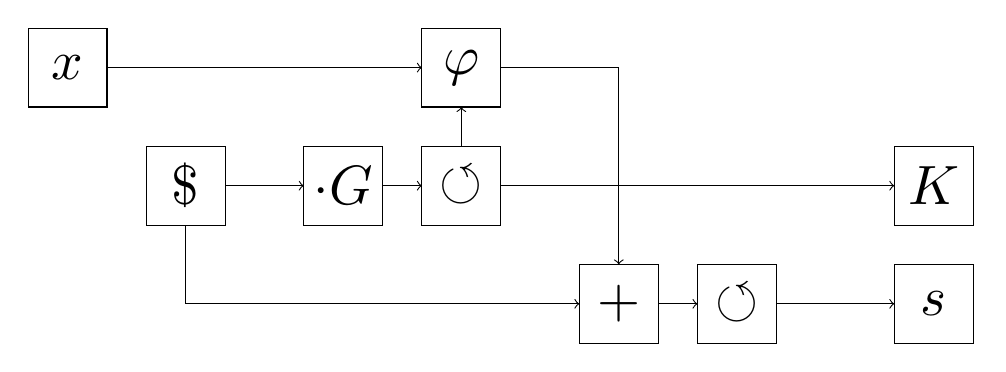
\begin{tikzpicture}[y=-1cm]
    \draw (0,0) rectangle (1,1) node[pos=0.5, scale=2.0] {$x$};
    \draw (1.5,1.5) rectangle (2.5,2.5) node[pos=0.5, scale=2.0] {$\$$};
    \draw (3.5,1.5) rectangle (4.5,2.5) node[pos=0.5, scale=2.0] {$\cdot G$};
    \draw (5.0,1.5) rectangle (6.0,2.5) node[pos=0.5, scale=2.0] {$\circlearrowleft$};
    \draw (5.0,0.0) rectangle (6.0,1) node[pos=0.5, scale=2.0] {$\varphi$};
    \draw (7.0,3.0) rectangle (8.0,4.0) node[pos=0.5, scale=2.0] {$+$};
    \draw (8.5,3.0) rectangle (9.5,4.0) node[pos=0.5, scale=2.0] {$\circlearrowleft$};
    \draw (11,3.0) rectangle (12,4.0) node[pos=0.5, scale=2.0] {$s$};
    \draw (11,1.5) rectangle (12,2.5) node[pos=0.5, scale=2.0] {$K$};
    \draw [->] (1, 0.5) -- (5.0, 0.5);
    \draw [->] (2.5, 2.0) -- (3.5, 2.0);
    \draw [->] (4.5, 2.0) -- (5.0, 2.0);
    \draw [->] (5.5, 1.5) -- (5.5, 1.0);
    \draw [->] (6.0, 2.0) -- (11, 2.0);
    \draw [->] (2.0, 2.5) -- (2.0, 3.5) -- (7.0, 3.5);
    \draw [->] (6.0, 0.5) -- (7.5, 0.5) -- (7.5, 3.0);
    \draw [->] (8.0, 3.5) -- (8.5, 3.5);
    \draw [->] (9.5, 3.5) -- (11, 3.5);
\end{tikzpicture}
\end{afigure}

Figure \ref{fig:schnorr} presents the circuit for Schnorr signatures,
with $\circlearrowleft$ denoting reconstruction nodes,
$\$$ denoting random input nodes, and $\varphi$ denoting
the parameterized homomorphism:

$$
\varphi(K)(x) := H(K, m) \cdot x
$$

Both the $\varphi$ and $+$ nodes have a depth of $2$, and thus so
does the circuit.

Using our semantics for circuits, we get a semi-honest protocol for
threshold Schnorr signatures. The quorum turns their threshold
secret sharing of the secret key $x$ into a linear secret sharing $\shared{x}$.
They then generate a shared nonce $\shared{k}$ by each sampling
$k_i \xleftarrow{R} \Zq$. They calculate a sharing $\shared{K := k \cdot G}$
by each computing $K_i := k_i \cdot G$. They then reveal these $K_i$ to
learn $K$. They can then compute $s_i := \varphi(K)(x_i)$ locally,
creating a sharing $\shared{s}$, whose shares they then reveal,
to learn $s$. They then use $(K, s)$ as their signature.

\subsection{Normalized Form}

While the formal definition of GRCs above is complete, and closely
matches the description of various functionalities, it's not
particularly convenient to design a protocol for.
We can vastly simplify the description of a GRC through the use
of a \emph{normalized form}, which is a much more compact representation
of this circuit.
This normalized form is also directly amenable to an implementation
as an MPC protocol.
This form is derived from a series of simple transformations on
a GRC.

First, note that the random input nodes of the GRC don't depend on
any other node. Because of this, we can move all of these input nodes
to the start of the circuit, which has the semantics of generating
all the randomness in the circuit at the start of the execution.

Second, instead of having several input nodes $x^1, \ldots, x^m$,
all elements of $\Zq$, we
instead have a single input \emph{vector} $\bx \in \Zq^m$.
This vector can also be considered as a single element of the product
group, with addition defined pointwise, as in Section \ref{sec:background}.
In fact, we can also include random elements as part of the input.
The idea is that honest parties will generate this part of the input
randomly for each execution.
We treat this issue in more detail in Section \ref{sec:idealfunc}.

Third, we can make each $\varphi$ node depend on the entire
input vector $\bx$.
In practice, this dependency can be sparse, in that $\varphi$
will only make use of a small number of elements in the input.
Nonetheless, $\varphi$ is still a homomorphism with respect
to the entire input.
This is because a projection $\pi : \Zq^m \to \Zq^l$, which selects
a subset of elements from an input vector, is a group homomorphism.
Any homomorphism using only a subset of elements can be composed with $\pi$
to make a homomorphism taking in the entire vector.

Fourth, we can coalesce the homomorphisms together, creating one
homomorphism for each ``layer'' of the circuit.
We do this by first organizing the $\varphi$ nodes into layers,
based on their depth.
Each node with the same depth goes into the same layer.
We then coalesce all of the homomorphisms in this layer into
a single homomorphism $\varphi$.
We can do this because the duplication map $a \mapsto (a, a)$
and the projection map $(a, \_) \mapsto a$ are both homomorphisms.
We can sort all of the homomorphisms topologically, and then compose
them sequentially, duplicating the input and projecting as necessary.

We can also remove reconstruction nodes.
Because each layer only has a single homomorphism, we can consider
the output of this homomorphism to neccessarily be reconstructed.
We then make each homomorphism parameterized by all of the reconstructed
outputs from each previous layer.

Finally, we can remove output nodes.
By considering the output of every layer to be part of the output,
we include all of the output nodes connected to reconstruction nodes.
For the other outputs, they can be locally computed using the reconstructed
outputs, as well as the shares of the input vector, so it's not necessary
to include them in the circuit.

Combining all of these gives us the formal description of normalized form
GRCs in Figure \ref{fig:grc}.

\begin{afigure}{fig:grc}{GRCs in normalized form}
A group reconstruction circuit (GRC) in normalized form consists of:
\begin{itemize}
    \item An input length $m$, and a depth $d$.
    \item Groups $\mathbb{B}_1, \ldots, \mathbb{B}_d$.
    \item Homomorphisms $\varphi_1, \ldots, \varphi_d$. Each $\varphi_i$
    is a homomorphism $\Zq^m \to \mathbb{B}_i$, and is parameterized
    by values $\bV_1, \ldots, \bV_{i - 1}$ with $\bV_i \in \mathbb{B}_i$.
\end{itemize}
\end{afigure}

We can also give circuits in this form semantics, in the form
of a semi-honest MPC protocol.
The parties have a linear secret sharing $\shared{\bx}$ of
the input vector, some entries of which having been generated randomly
for this execution.
Then, for each layer $r \in 1, \ldots, d$, the parties locally
compute $\bV_r^i := \varphi_r(\bV_1, \ldots, \bV_{r - 1})$,
and then reveal these shares, allowing each party to compute
$\bV_r := \sum_i \bV_r^i$.
The values $\bV_1, \ldots, \bV_d$ make up the output of the protocol.

In Section \ref{sec:applications}, we provide examples of GRCs
in normalized form for several functionalities, including Schnorr
signatures.

\section{MPC Protocol for GRCs}

In this section, we describe an MPC protocol for computing
a GRC on linearly shared inputs, with associated commitments.
We also analyze the security of this protocol, proving that it
is secure against an arbitrary number of malicious parties,
and under concurrent composition, in the UC framework.

For inputs, one natural kind of commitment are Pedersen commitments.
In many protocols, however, it's more natural to use plain commitments,
where a scalar $x$ is committed to with the value $x \cdot G$.
This matches most threshold Schnorr schemes,
in which the secret $x$ is split into shares $x_i$, with the shares
of the public key $X_i := x_i \cdot G$ being known for all parties.
While we could subsume these commitments as a case of Pedersen commitments,
with a blinding factor set to $0$, explicitly considering these
plain commitments yields a more efficient protocol.

We thus split our input vector into three sections: $\bx, \by, \bk$.
Each of this is linearly split into shares.
We have shares $\bx^1, \ldots, \bx^n$ for each party, such that $\bx = \sum_i \bx^i$,
and similarly for $\by$ and $\bk$.
The shares of $\bx$ have plain commitments $\bX^i = \bx_i \cdot G$
for each party.
The shares of $\by$ have Pedersen commitments $\bY^i = \by_i \cdot G + \balpha^i \cdot H$,
with $\balpha^i$ a vector of blinding factors held by each party.
Finally, $\bk$ is intended to be randomly generated for each execution
of the protocol.
Honest parties will generate their share $\bk^i$ by sampling a random
vector.
As long as at least one participant in the protocol is honest,
then $\bk := \sum_i \bk^i$ will also be random.

\subsection{Ideal Functionality}
\label{sec:idealfunc}
In this section, we describe an ideal functionality for our protocol,
as Functionality \ref{fun:mpc}.
This functionality is parameterized by the circuit $\Phi$,
as well as the input commitments $\bX^i$ and $\bY^i$, for each party
$i \in [n]$.
The functionality also uses a common reference string $(G, H) \in \mathbb{G}^2$,
for Pedersen commitments.

\begin{afunctionality}{fun:mpc}{GRC functionality $\mathcal{F}(\texttt{GRC}, \Phi, \textbf{X}^i, \textbf{Y}^i)$}
A functionality $\mathcal{F}$ for parties $P_1, \ldots, P_n$.\\
\\
After receiving
$(\texttt{input}, \texttt{sid}, \textbf{x}^i, \textbf{y}^i, \boldsymbol{\alpha}^i, \textbf{k}^i)$ from every party $P_i$:\\
$\mathcal{F}$ checks, for every $i \in [n]$, that:
$$
\begin{aligned}
    \textbf{X}^i &\stackrel{?}{=} \textbf{x}^i \cdot G\\
    \textbf{Y}^i &\stackrel{?}{=} \textbf{y}^i \cdot G + \boldsymbol{\alpha}^i \cdot H\\
\end{aligned}
$$
$\mathcal{F}$ computes, for each round $r \in [d]$:
$$
\begin{aligned}
    \textbf{V}^i_{r} &:= \varphi_{r}(\textbf{V}_{1}, \ldots, \textbf{V}_{r - 1})(
        \textbf{x}^i, \textbf{y}^i, \textbf{k}^i
    )\\
    \textbf{V}_r &:= \sum_j \textbf{V}^i_r
\end{aligned}
$$\\
$\mathcal{F}$ sends $(\texttt{output}, \texttt{sid}, \textbf{V}^1_1, \ldots, \textbf{V}^n_d)$ to every party $P_i$.
\end{afunctionality}

This functionality checks that the inputs each party provides match
the public commitments, and then computes the output of the circuit
in a straightforward manner.
One slight difference is that instead of simply learning $\bV_r$ for
every round $r$, each party learns $\bV^i_r$ for every party $i$.
Naturally, we have $\bV_r = \sum_i \bV^i_r$, so this information
can be derived by each party.
The reason we allow the parties to also learn the individual shares
being revealed is that our eventual protocol will also reveal this
information, so we need to model the leakage in our functionality as well.
Furthermore, this matches the semantics of group reconstruction circuits,
where parties learn the individual shares of the group element they're
reconstructing.
For practical functionalities like Schnorr signatures or threshold encryption,
learning these intermediate values is not a concern either.

\subsection{Protocol}

In this section, we provide a protocol implementing Functionality
\ref{fun:mpc}.

The basic idea is that for each round $r$, the parties locally
compute $\bV^i_r := \varphi_r(\bx^i, \by^i, \bk^i)$, and then
send these values to other parties, along with a proof that
the value was computed correctly, and that the inputs used correspond
to the public commitments.

For the random input $\bk^i$, we need to guarantee that the same
input vector is used throughout the protocol.
We do this by creating a Pedersen commitment $\bK^i$ to the random value,
and having an initial round where each party broadcasts this commitment
to the other parties.
To prevent a party from sending different commitments, we
use Functionality \ref{fun:broadcast} to guarantee that the same
commitment is sent to all parties.

We can easily prove that each step was computed correctly, and with the right
inputs, by using the following homomorphism:
$$
\psi_r(\textbf{x}, \textbf{y}, \boldsymbol{\alpha}, \textbf{k}, \boldsymbol{\beta})
:= (\varphi_r(\bx, \by, \bk),\ \bx \cdot G,\ \by \cdot G + \balpha \cdot H,\
\bk \cdot G + \bbeta \cdot H) 
$$
This homomorphism uses the same inputs to compute $\varphi_r$,
but also reconstructs all of the commitments to the inputs.
The $\varphi$-proofs seen in Section \ref{sec:maurer}
provide an efficient sigma protocol to verify
that a value $\bV^i_r$ was computed using $\varphi_r$ on the correct
inputs.
We then use Functionality \ref{fun:zk} to turn these sigma protocols
into ZK proof of knowledge functionalities.

Protocol \ref{prot:mpc} describes all of this more formally.
Like the ideal functionality, the protocol is parameterized by
the circuit $\Phi$, the public commitments $\bX^i, \bY^i$, and makes
use of a common reference string $(G, H) \in \mathbb{G}^2$, for Pedersen
commitments.
The protocol takes $d + 1$ rounds, with $d$ the depth of the circuit.
As we mentioned in the previous section, the parties learn
the intermediate values $\bV^i_r$ as a consequence of the protocol's
execution.

\begin{aprotocol}{prot:mpc}{MPC protocol for $\Phi, \textbf{X}^i, \textbf{Y}^i$}

Each party $P_i$ has inputs $\textbf{x}^i$ and $\textbf{y}^i$, committed to
by $\textbf{X}^i$ and $\textbf{Y}^i$.
They also have decommitments $\boldsymbol{\alpha}^i$ for $\textbf{Y}^i$.
Each party $P_i$ also has a vector $\textbf{k}^i$, which honest parties will
have generated randomly.\\
\\
\textbf{Round 0}\\
Each party $P_i$ generates a random vector $\boldsymbol{\beta}^i$, and creates
a commitment to $\textbf{k}^i$ with:
$$
\textbf{K}^i := \bk^i \cdot G + \bbeta^i \cdot H
$$
$P_i$ sends $(\texttt{broadcast-in}, \texttt{sid}, \textbf{K}^i)$ to
the broadcast functionality $\mathcal{C}$.\\
$P_i$ waits to receive $(\texttt{broadcast-out}, \texttt{sid}, \textbf{K}^j)$
for each other party $j$.\\
\\
\textbf{Round $r$}\\
Each party $P_i$ computes $\bV^i_r := \varphi_r(\bV_1, \ldots, \bV_{r - 1})(\bx^i, \by^i, \bk^i)$.\\
Each party $P_i$ sends $(\texttt{prove}, \texttt{sid}, (\bx^i, \by^i, \balpha^i, \bk^i, \bbeta^i))$
to $\mathcal{F}(\texttt{ZK}, \psi_r)$, receiving $\pi^i_r$ in return.\\
Each party $P_i$ sends $(\bV^i_r, \pi^i_r)$ to every other party.\\
\\
After receiving $(\bV^j_r, \pi^j_r)$  from all other parties, $P_i$ checks,
for each $j$, that the proof is valid, by sending $(\texttt{verify}, (\bV^j_r, \bX^j, \bY^j, \bK^j), \pi^j_r)$ to
$\mathcal{F}(\texttt{ZK}, \psi_r)$, and aborting if the functionality returns $0$.\\
Each party $P_i$ then stores each $\bV^j_r$ as part of its output,
and computes $\bV_r := \sum_j \bV^j_r$.
\end{aprotocol}

\subsection{Security Analysis}

In this section, we prove that Protocol \ref{prot:mpc} implements
Functionality \ref{fun:mpc} with UC security, even against an arbitrary
number of malicious parties.
More specifically, we work with the SUC model of security~\cite{canetti_simpler_2015}.
We also work in the hybrid model, using Functionalities
\ref{fun:zk} and \ref{fun:broadcast} for ZK proofs of knowledge,
and authenticated broadcast, respectively.
We also need a common reference string $(G, H) \in \mathbb{G}^2$, for
Pedersen commitments.
In our proof, the simulator provides this string.

\begin{claim}
Provided that the discrete logarithm is hard in $\mathbb{G}$, Protocol \ref{prot:mpc} securely implements Functionality \ref{fun:mpc},
in the hybrid model of universally composable security,
given a zk functionality $\mathcal{F}(\text{ZK}, \varphi)$ (for arbitrary $\varphi$),
a broadcast functionality $\mathcal{C}$, as well as a common reference string
${(G, H) \in \mathbb{G}^2}$.
\end{claim}
\textbf{Proof Idea:}\\
The basic idea is that we use an instance of the discrete logarithm problem
as our common reference string.
This makes any break of the binding property of Pedersen commitments
yield a solution to the discrete logarithm.
Otherwise, we can perfectly simulate an execution of the protocol
using the ideal functionality, without rewinding
the adversary, which lets us conclude that our protocol is UC secure,
using the result in \cite{kushilevitz_information-theoretically_2009}.

One technical detail is that we need inputs from every party
to give to the ideal functionality.
Because of this, our simulator first runs the simulated protocol
until the adversary provides the input for their parties in the first
ZK proof.
We can then use these values for the parties the simulator controls
in the ideal functionality.

The output of this functionality gives us all of the values we need
in the rest of the simulation, except for the commitments $\bK^i$
to the random inputs of the honest parties.
For these, we use the fact that Pedersen commitments are perfectly
hiding, and simply generate them at random.

\textbf{Proof:}\\
We prove this by constructing a simulator $\calS$ which uses
the ideal functionality $\mathcal{F}(\texttt{GRC})$ to perfectly
simulate an execution of the hybrid protocol against an adversary
$\mathcal{A}$.

We also work in the common reference string model, where the simulator
$\mathcal{S}$ chooses the bases $(G, H)$ for the Pedersen commitments.

We use this simulator $\calS$ to construct an adversary against
the discrete logarithm game.

Let $\calM \subseteq \calP$ be the set of malicious parties,
and $\calH \subseteq \calP$ be the set of honest parties. Naturally,
we have $\calH \cup \calM = \calP$ and $\calH \cap \calM = \emptyset$.

As an adversary against the discrete logarithm game,
$\calS$ receives $(G, H)$ as an instance 
of the discrete logarithm problem.

The simulator then proceeds as follows:\\
$\calS$ starts by setting $(G, H)$ as the common reference string.

\textbf{Round 0}:\\
For each $i \in \calH$, $\calS$ samples $\bK^i \xleftarrow{R} \mathbb{G}$.\\
For each $i \in \calM$,
$\calS$ waits to receive $(\texttt{broadcast-in}, \texttt{sid}, \bK^i)$.\\
$\calS$ then sends $(\texttt{broadcast-out}, \texttt{pid}_i, \texttt{sid}, \bK^i)$,
to all parties, for every $i \in \calP$, emulating $\mathcal{C}$.

\textbf{Interim}:\\
$\calS$ waits to receive $(\texttt{prove}, \texttt{sid}, (\bx^i, \by^i, \balpha^i, \bk^i, \bbeta^i))$
for each malicious ${i \in \calM}$,
playing the role of $\mathcal{F}(\texttt{ZK}, \psi_1)$.\\
$\calS$ checks, for each $i$, that:
$$
\begin{aligned}
\bX^i &\stackrel{?}{=} \bx^i \cdot G\\
\bY^i &\stackrel{?}{=} \by^i \cdot G + \balpha^i \cdot H\\
\bK^i &\stackrel{?}{=} \bk^i \cdot G + \bbeta^i \cdot H
\end{aligned}
$$
otherwise, $\calS$ sets $\texttt{bad-values}^i_1 \gets 1$.\\
$\calS$ records the values $\bx^i, \by^i, \balpha^i, \bk^i, \balpha^i$, for $i \in \calM$.\\

Now, in the real execution against $\mathcal{F}(\texttt{GRC})$,
with real honest parties $P_i$, for
each $i \in \calM$, the parties $\calS$ controls, $\calS$ sends
$(\texttt{input}, \texttt{sid}, \bx^i, \by^i, \balpha^i, \bk^i)$ to $\mathcal{F}(\texttt{GRC})$.\\
$\calS$ receives $(\texttt{output}, \texttt{sid}, \bV^1_1, \ldots, \bV^n_d)$ in return,
and records these values.

\textbf{Round $r$}:\\
For each round $r \in [d]$, $\calS$ proceeds as follows:\\
$\calS$ generates a new $\pi^j_r$ for each $j \in \calH$, and sends
$(\bV^j_r, \pi^j_r)$ to every malicious $P_i$, with $i \in \calM$.

Unless $r = 1$, $\calS$ waits to receive 
$(\texttt{prove}, \texttt{sid}, \hat{\bx}^i, \hat{\by}^i, \hat{\balpha}^i, \hat{\bk}^i, \hat{\bbeta}^i)$
from each malicious $P_i$, for $i \in \calM$, playing the role of $\mathcal{F}(\texttt{ZK}, \psi_r)$.\\
$\mathcal{S}$ then checks, for each $i$, that:
$$
\begin{aligned}
\bX^i &\stackrel{?}{=} \hat{\bx}^i \cdot G\\
\bY^i &\stackrel{?}{=} \hat{\by}^i \cdot G + \hat{\balpha}^i \cdot H\\
\bK^i &\stackrel{?}{=} \hat{\bk}^i \cdot G + \hat{\bbeta}^i \cdot H
\end{aligned}
$$
and sets $\texttt{bad-values}^i_r \gets 1$ otherwise.\\
The first check implies that $\hat{\bx^i} = \bx^i$. If it holds that
$\hat{\by}^i \neq \by^i$ or $\hat{\bk}^i \neq \bk^i$, then $\calS$ has
found a value $h$ such that $h \cdot G = H$, as per Claim \ref{claim:ped_vec_dlog},
and $\calS$ aborts, returning $h$.

(Including when $r = 1$) $\calS$ generates a new $\pi^i_r$, and returns $(\texttt{proof}, \pi^i_r)$,
playing the role of $\mathcal{F}(\texttt{ZK}, \psi_r)$.

Concurrently, $\calS$ plays the role of $\mathcal{F}(\texttt{ZK}, \psi_r)$,
responding to $(\texttt{verify}, (\hat{\bV}^j_r, \hat{\bX}^j, \hat{\bY}^j, \hat{\bK}^j), \pi)$
queries. $\calS$ checks that there exists some $i \in \mathcal{P}$ such that
$\pi^i_r = \pi$. $\calS$ then returns:
$$
\hat{\bV}^j_r \stackrel{?}{=} \bV^j_r \land
\hat{\bX}^j \stackrel{?}{=} \bX^j \land
\hat{\bY}^j \stackrel{?}{=} \bY^j \land
\hat{\bK}^j \stackrel{?}{=} \bK^j \land
\texttt{bad-values}^i_r \neq 1
$$

$\calS$ then waits to receive $(\hat{\bV}^i, \hat{\pi}^i_r)$ for
every malicious party $P_i$, with ${i \in \mathcal{M}}$.\\
$\calS$ then checks if the query $(\texttt{verify}, (\hat{\bV^i_r}, \bX^i, \bY^i, \bK^i), \hat{\pi}^i_r)$
would yield $1$, according to the logic in the section above.
(If $\hat{\pi}^i_r$ doesn't match anything, the check is considered to fail).
If this check fails, then $\calS$ simulates every honest $P_j$ aborting, with $j \in \calH$,
to abort, as if they'd seen an invalid proof themselves.

This concludes the simulation.

If $\calS$ aborts with a value $h$, then they've successfully
solved an instance of the discrete logarithm problem. Under our
assumption that this problem is hard, this happens with negligeable
probability.

We argue that if $\calS$ does not abort in this way, then the simulation
is perfect. For the first round, because pedersen commitments
are perfectly hiding, sampling a random $\bK^i$ has an identical
distribution as an honest party generating a pedersen commitment.
For the rest of the protocol, all of our checks are equivalent
to those made by honest parties. This is because the
$\bV^j_i$ values are necessarily computed correctly, and use
the inputs provided by the parties the adversary $\mathcal{A}$ controls.

Because our simulator $\calS$ is perfect, and doesn't
rewind the adversary $\mathcal{A}$, we conclude,
using~\cite{kushilevitz_information-theoretically_2009},
that our protocol
satisfies universally composable security, in the hybrid model.

$\blacksquare$

\subsubsection{Identifiable Abort}

We note that our protocol can be considered to have identifiable
aborts, provided that the implementation of the broadcast functionality
also has this property.
After round $0$, if a party causes an abort by providing an invalid
proof, then that abort can be detected, since there will be
a signed message containing this invalid proof, which can be used
as evidence of cheating.

\subsection{Practical Considerations}

In this section we describe a few additional details which might
be useful for concrete implementations of the protocol.

\subsubsection{Sparse Proofs}

\subsubsection{Parallel Echos}

\subsubsection{Parallel $\texttt{sid}$}

\subsection{Concrete Complexity}

\section{Applications}
\label{sec:applications}

\todo{One example application for DKG, Schnorr, Threshold Encryption, Polynomial Commitments}

\section{Limitations and Further Work}

\todo{Aggregating proofs}

\todo{Exploiting circuit structure for lighter proofs}

\todo{Threshold Interpretations}

\section{Conclusion}

\todo{Summarize stuff}

\bibliographystyle{alpha}
\small \bibliography{bib}
\end{document}
